%----------------------------------------------------------------------------------------
% METADATA BLOCK (YAML)  — see inbox/README.md for every field
%----------------------------------------------------------------------------------------
% uid: ""
% school: "lycee"
% level: "3eme"
% section: "Mathématiques"
% chapter: "Nombres complexes"
% title: "Droite de Simson, droite de Steiner"
% difficulty: "Difficile"
% tags: ["simson", "steiner", "nombres-complexes", "cercle-unite", "orthocentre"]
% provenance: "adapted"
% batch: "2026-11-20-defis-geometrie-A"
%----------------------------------------------------------------------------------------

\newcommand{\R}{\mathbb{R}}
\newcommand{\C}{\mathbb{C}}

% ---STATEMENT---
Le plan est identifié à $\C$. Soit $ABC$ un triangle inscrit dans le cercle unité $\{z\in\C,\ |z|=1\}$ ; $a$, $b$, $c$ sont les affixes de $A$, $B$, $C$ (distincts, de module $1$). On rappelle que $\bar z=\dfrac1z$ lorsque $|z|=1$.
Soit $P$ un point du cercle, distinct de $A$, $B$, $C$, d'affixe $p$.

% alt: Cercle circonscrit, point P du cercle, projetés orthogonaux D, E, F sur les trois côtés alignés (droite de Simson)
\begin{center}
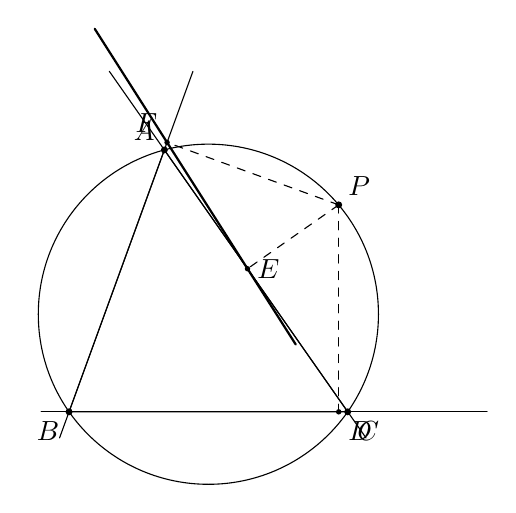
\begin{tikzpicture}[scale=0.9,line cap=round,line join=round,>=stealth]
\draw (0,0) circle (2.4);
\draw (-0.621,2.318) -- (-1.966,-1.377) -- (1.966,-1.377) -- cycle;
\draw[thin] (-2.359,-1.377) -- (3.932,-1.377);
\draw[thin] (2.225,-1.746) -- (-1.397,3.427);
\draw[thin] (-0.218,3.427) -- (-2.1,-1.746);
\draw[dashed] (1.839,1.543) -- (1.839,-1.377);
\draw[dashed] (1.839,1.543) -- (0.552,0.642);
\draw[dashed] (1.839,1.543) -- (-0.583,2.424);
\draw[thick] (1.233,-0.427) -- (-1.604,4.028);
\fill(-0.621,2.318) circle (1.4pt) node[above left] {$A$};
\fill(-1.966,-1.377) circle (1.4pt) node[below left] {$B$};
\fill(1.966,-1.377) circle (1.4pt) node[below right] {$C$};
\fill(1.839,1.543) circle (1.4pt) node[above right] {$P$};
\fill(1.839,-1.377) circle (1.1pt) node[below right] {$D$};
\fill(0.552,0.642) circle (1.1pt) node[right] {$E$};
\fill(-0.583,2.424) circle (1.1pt) node[above left] {$F$};
\end{tikzpicture}
\end{center}

\begin{enumerate}
  \item \textbf{Projeté orthogonal.} Montrer qu'un point $M(z)$ appartient à la droite $(BC)$ si et seulement si $z+bc\,\bar z=b+c$.
  \item Montrer que le projeté orthogonal $D$ de $P$ sur $(BC)$ a pour affixe $d=\dfrac12\left(p+b+c-bc\,\bar p\right)$. On note $E$ et $F$ les projetés orthogonaux de $P$ sur $(CA)$ et $(AB)$ : donner leurs affixes $e$ et $f$.
  \item \textbf{Droite de Simson.} Calculer $d-e$ et $d-f$, puis montrer que \textbf{les projetés $D$, $E$, $F$ de $P$ sur les trois côtés sont alignés}.
  \item \textbf{Droite de Steiner.} Soient $P_a$, $P_b$, $P_c$ les symétriques de $P$ par rapport aux droites $(BC)$, $(CA)$, $(AB)$. Montrer que \textbf{$P_a$, $P_b$, $P_c$ sont alignés}.
  \item
  \begin{enumerate}
    \item Vérifier que le point $H$ d'affixe $h=a+b+c$ est l'orthocentre de $ABC$.
    \item Montrer que \textbf{la droite $(P_aP_b)$ passe par $H$.}
  \end{enumerate}
\end{enumerate}

\emph{Remarque (sans démonstration demandée).} Lorsque $P$ décrit le cercle, les droites de Simson enveloppent une deltoïde (hypocycloïde à trois rebroussements) dont le cercle inscrit est le cercle d'Euler de $ABC$.

% ---SOLUTION---
\begin{enumerate}[itemsep=14pt]
  \item\leavevmode
  \begin{prop}[Alignement et perpendicularité en complexes]
  $M(z)$, $B(b)$, $C(c)$ sont alignés si et seulement si \ib{$\dfrac{z-b}{c-b}\in\R$}.

  Les vecteurs d'affixes $u$ et $v\neq0$ sont orthogonaux si et seulement si \ib{$\dfrac uv\in i\R$} (imaginaire pur).

  Un nombre $w$ est réel si et seulement si $\bar w=w$ ; il est imaginaire pur si et seulement si $\bar w=-w$.
  \end{prop}
  $M\in(BC)\iff\dfrac{z-b}{c-b}=\overline{\left(\dfrac{z-b}{c-b}\right)}=\dfrac{\bar z-\bar b}{\bar c-\bar b}$.

  Or $\bar c-\bar b=\dfrac1c-\dfrac1b=\dfrac{b-c}{bc}$ et $\bar b=\dfrac1b$. Donc
  \[\dfrac{z-b}{c-b}=\dfrac{\bar z-\frac1b}{\frac{b-c}{bc}}=-bc\,\dfrac{\bar z-\frac1b}{c-b}.\]
  On simplifie par $c-b\neq0$ : $z-b=-bc\,\bar z+c$, c'est-à-dire \ib{$z+bc\,\bar z=b+c$}.

  \item Le projeté $D(d)$ vérifie deux conditions.

  \emph{(i) $D\in(BC)$ :} $d+bc\,\bar d=b+c$.

  \emph{(ii) $(PD)\perp(BC)$ :} $\dfrac{p-d}{b-c}$ est imaginaire pur. Son conjugué vaut
  \[\dfrac{\bar p-\bar d}{\bar b-\bar c}=\dfrac{\bar p-\bar d}{\frac{c-b}{bc}}=-bc\,\dfrac{\bar p-\bar d}{b-c},\]
  et il doit être l'opposé de $\dfrac{p-d}{b-c}$ : $p-d=bc\,(\bar p-\bar d)$, soit $d-bc\,\bar d=p-bc\,\bar p$.

  On additionne (i) et (ii) : $2d=p+b+c-bc\,\bar p$, donc \textbf{$d=\dfrac12\left(p+b+c-bc\,\bar p\right)$}.

  Par permutation circulaire $(a,b,c)\to(b,c,a)$ :
  \[e=\dfrac12\left(p+c+a-ca\,\bar p\right),\qquad f=\dfrac12\left(p+a+b-ab\,\bar p\right).\]

  \item On calcule :
  \[d-e=\dfrac12\left[(b-a)-c(b-a)\bar p\right]=\dfrac12(b-a)(1-c\,\bar p),\qquad d-f=\dfrac12(c-a)(1-b\,\bar p).\]
  Comme $\bar p=\dfrac1p$ : $1-c\bar p=\dfrac{p-c}{p}$ et $1-b\bar p=\dfrac{p-b}{p}$. Donc
  \[Z=\dfrac{d-e}{d-f}=\dfrac{(b-a)(p-c)}{(c-a)(p-b)}.\]
  Pour des nombres de module $1$ : $\overline{u-v}=\dfrac1u-\dfrac1v=\dfrac{v-u}{uv}$. On conjugue chaque facteur :
  \[\bar Z=\dfrac{\frac{a-b}{ab}\cdot\frac{c-p}{cp}}{\frac{a-c}{ac}\cdot\frac{b-p}{bp}}=\dfrac{(a-b)(c-p)}{(a-c)(b-p)}\times\dfrac{ac\cdot bp}{ab\cdot cp}=\dfrac{(a-b)(c-p)}{(a-c)(b-p)}=Z.\]
  $Z$ est réel : \ib{$D$, $E$, $F$ sont alignés}.

  \item\leavevmode
  \begin{prop}[Symétrie et homothétie]
  Le symétrique de $P$ par rapport à une droite est l'image de $P$ par l'homothétie de centre $P$ et de rapport $2$ appliquée au projeté orthogonal de $P$ sur cette droite. Une homothétie conserve l'alignement.
  \end{prop}
  $D$ est le milieu de $[PP_a]$ : $P_a=2d-p=b+c-bc\,\bar p$. De même $P_b=2e-p$ et $P_c=2f-p$.

  Ainsi $P_a$, $P_b$, $P_c$ sont les images de $D$, $E$, $F$ par l'homothétie $h(P,2)$. Comme $D$, $E$, $F$ sont alignés, \ib{$P_a$, $P_b$, $P_c$ sont alignés}.

  \item
  \begin{enumerate}[itemsep=8pt]
    \item $\dfrac{h-a}{b-c}=\dfrac{b+c}{b-c}$. Son conjugué est $\dfrac{\frac1b+\frac1c}{\frac1b-\frac1c}=\dfrac{c+b}{c-b}=-\dfrac{b+c}{b-c}$ : ce nombre est imaginaire pur, donc $(AH)\perp(BC)$.

    Les affixes sont symétriques en $a,b,c$ : $H$ est aussi sur les hauteurs issues de $B$ et $C$. $H$ est l'orthocentre.
    \item Avec $P_a=b+c-\dfrac{bc}p$ et $P_b=c+a-\dfrac{ca}p$ :
    \[h-P_a=a+\dfrac{bc}p=\dfrac{ap+bc}{p},\qquad h-P_b=b+\dfrac{ca}p=\dfrac{bp+ca}{p}.\]
    Soit $W=\dfrac{h-P_a}{h-P_b}=\dfrac{ap+bc}{bp+ca}$. On conjugue :
    \[\overline{ap+bc}=\dfrac1{ap}+\dfrac1{bc}=\dfrac{bc+ap}{abcp},\qquad\overline{bp+ca}=\dfrac1{bp}+\dfrac1{ca}=\dfrac{ca+bp}{abcp}.\]
    Donc $\bar W=W$ : $W$ est réel, et \ib{$H\in(P_aP_b)$}. $\blacksquare$
  \end{enumerate}
\end{enumerate}

\textbf{Remarque (réciproque de Simson).} Pour $p$ quelconque, $d-e=\dfrac12(b-a)(1-c\bar p)$ et $d-f=\dfrac12(c-a)(1-b\bar p)$. En conjuguant comme ci-dessus (seuls $a,b,c$ sont de module $1$), $\bar Z=\dfrac{b-a}{c-a}\cdot\dfrac{c-p}{b-p}$. Donc $Z$ est réel si et seulement si $(b-p)(1-c\bar p)=(c-p)(1-b\bar p)$, soit $(b-c)(1-|p|^2)=0$ : \emph{les projetés de $P$ sont alignés si et seulement si $P$ est sur le cercle circonscrit.}

\textbf{Idée :} avec $\bar z=\dfrac1z$ sur le cercle unité, la géométrie devient de l'algèbre. La droite de Simson est l'image de la droite de Steiner par l'homothétie de centre $P$ et de rapport $\dfrac12$ ; elle passe donc par le milieu de $[PH]$, qui est sur le cercle d'Euler.

\textbf{Piège :} la formule $d=\dfrac12(p+b+c-bc\bar p)$ est vraie pour tout $p$, mais la simplification $1-c\bar p=\dfrac{p-c}{p}$ n'est valable que si $|p|=1$.
